\chapter{Organizational and People Issues}

This session from Joseph Hadzima's MIT OpenCourseWare course is not a doctrinal lecture but an interactive panel on how ventures are actually held together. That matters for the way we should write it. The argument does not proceed by a single theory of organizations. It proceeds by tension, question, example, correction, and return. The mathematics is correspondingly modest but still real. It appears here as threshold logic, scaling examples, decision rules, and compact tests for when an organization has crossed from structure into obstruction. These notes follow the transcript closely and are curated for book form by LazyingArt LLC.

\section{People Issues As The Dominant Failure Mode}

Hadzima begins by recalling the first day of the course. A new venture requires several elements to come together, but the present session narrows the field sharply. The factor most likely to sink the venture is not the technology and not the funding. It is the people side of the enterprise. We should read that as an ordering of practical causes, not as a numerical claim.

\begin{equation}
\text{people issues} \succ \text{technology},
\qquad
\text{people issues} \succ \text{funding}.
\end{equation}

That ordering explains the form of the evening. If the principal failure mode is human rather than purely technical, then a panel is more useful than a sermon. Vivian moderates. One panelist speaks from founder-scale people building and boards. Another speaks from large-company HR and acquisition. A third brings process and operations design. The room is then invited to interrupt, ask, challenge, and refine. The lecture's rhythm is therefore not accidental. It is part of the teaching method.

\begin{remark}
The displayed formulas in this chapter are transcript-backed heuristics rather than board equations from the room. They are included only to make the lecture's operating logic visible.
\end{remark}

The opening claim also gives the chapter its tone. We are not dealing with ``soft'' material in the dismissive sense. The whole session argues the opposite. People are not one more function inside the company. They are the medium through which every other function is executed, delayed, clarified, or spoiled.

\section{Culture Starts Before HR}

The first substantive correction in the panel is decisive. Culture does not begin when a company finally hires an HR person. It begins at founding. Before any formal department exists, the founders have already started defining the company: what matters, how quality is judged, how they speak to one another, what behavior is rewarded, how mistakes are handled, and whether trust is real or merely assumed.

The lecture returns several times to a small set of early mechanisms.

\begin{enumerate}
\item founders must speak explicitly about what is important;
\item trust must be present in seed form and then built in practice;
\item hiring behavior already creates culture;
\item routine gives the company cadence and therefore security.
\end{enumerate}

The point about routine is worth pausing over, because the panel gives it more weight than a reader might expect. Vivian compares management to parenting in one narrow but useful sense: regular routines do not merely organize time, they stabilize a human environment. In a tiny company, this matters. If everything is improvised, every error feels existential. If there is cadence, then the company can make mistakes without dissolving into panic.

\subsection{Question \& Answer}

\paragraph{Question.} When should we start thinking about the HR function, and how do we preserve the company's DNA as investors arrive?

\paragraph{Answer.} The answer is earlier and later than one might think. Earlier, because the real content of culture begins immediately. Later, because the formal function often comes after founders, advisors, and a small set of routines have already carried the organization through its first stage.

Let \(n\) denote headcount, and let \(\operatorname{support}(n)\) denote the amount of explicit people and organizational support the company requires at stage \(n\). A fair compression of the panel's threshold logic is

\begin{equation}
\operatorname{support}(n)=
\begin{cases}
\text{founder-led / informal}, & n<25,\\
\text{outside guidance useful}, & 25\le n\le 50,\\
\text{explicit people support hard to avoid}, & n\gtrsim 50.
\end{cases}
\end{equation}

This is a heuristic, not a law. The exact threshold depends on the business. But the lecture is plain that somewhere around the \(25\) to \(50\) range outside help becomes materially useful, and by roughly \(50\) people the company is usually beyond pure improvisation.

\paragraph{Worked example.} The value of the heuristic is not predictive precision. Its value is that it makes regime change visible.

\begin{align}
n=12 &\Rightarrow \operatorname{support}(n)=\text{founder-led / informal},\\
n=35 &\Rightarrow \operatorname{support}(n)=\text{outside guidance useful},\\
n=60 &\Rightarrow \operatorname{support}(n)=\text{explicit people support becomes urgent}.
\end{align}

At \(n=12\), founder attention, trust, and routine still carry most of the load. At \(n=35\), legal, financial, and organizational advice become useful. At \(n=60\), the firm can no longer assume that role design, fairness, and people process will take care of themselves.

\begin{figure}
\centering
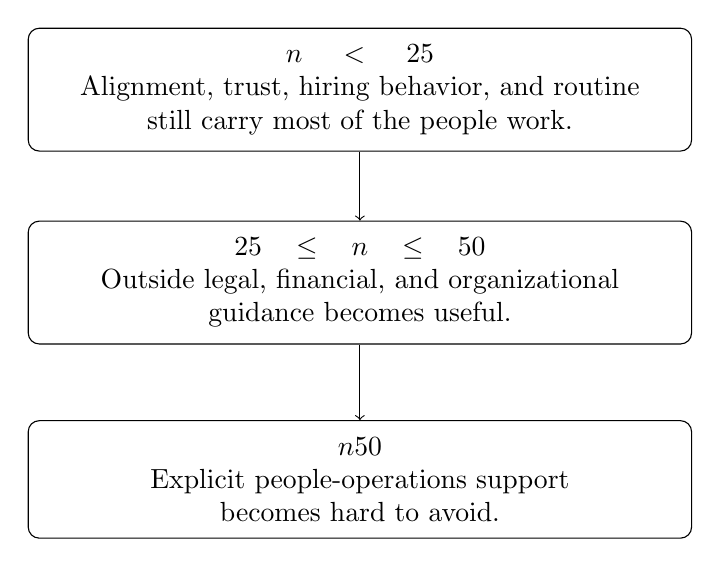
\begin{tikzpicture}
\node[draw, rounded corners, align=center, text width=0.66\linewidth, inner sep=6pt] (a) at (0,0) {$n<25$\\Alignment, trust, hiring behavior, and routine\\still carry most of the people work.};
\node[draw, rounded corners, align=center, text width=0.66\linewidth, inner sep=6pt] (b) at (0,-2.45) {$25\le n\le 50$\\Outside legal, financial, and organizational\\guidance becomes useful.};
\node[draw, rounded corners, align=center, text width=0.66\linewidth, inner sep=6pt] (c) at (0,-4.95) {$n\gtrsim 50$\\Explicit people-operations support\\becomes hard to avoid.};
\draw[->] (a.south) -- (b.north);
\draw[->] (b.south) -- (c.north);
\end{tikzpicture}
\caption{Transcript-derived stage heuristic for people and organizational support. The lecture presents these as rough thresholds, not exact boundaries.}
\end{figure}

The panel then adds two practical refinements. First, early companies often bring in legal or financial help before they bring in a human-resources specialist, because payroll, taxes, and basic financial control become urgent quickly. Second, once the people function does arrive, it should not simply disappear under finance. The lecture is unusually direct here: do not make HR a shadow of the finance office. The functions are connected, but not identical.

\paragraph{Stage and scale.} At this point the panel turns from timing to meaning. The question is no longer only when support becomes necessary. It becomes what sort of company is being supported. Two scale markers sharpen the point:

\begin{align}
n_{\mathrm{RSA}} &: 55 \rightarrow 2000,\\
n_{\mathrm{Thermo}} &\approx 130000.
\end{align}

The RSA example is used to show stage dependence. A company that moves from roughly \(55\) people to roughly \(2{,}000\) does not remain organizationally unchanged. At each stage of growth, different things are needed. But the values can remain stable across those changes. The Thermo Fisher example shows something complementary: even at very large scale, a simple mission can still bind the organization. The point is not sloganism. The point is that dispersed tasks must still be legible to the people performing them.

This is why the lecture immediately resists a false opposition. Vivian says that the organizations she most admired combined high achievement with human kindness. High standards were not softened. What mattered was that there was still a human way of doing difficult things. Even layoffs or structural changes could be carried out with respect.

\paragraph{Example.} Michelle's ``people first'' company makes the same point from another angle. The founder's rule was simple: if you take care of your people, your people take care of your customers, and the rest has a chance to work. That is not sentimentality. It is a theory of organizational transmission. Customer treatment, revenue generation, and retention of talent are not separate lines. They are linked.

\section{Roles, Friendship, And The Co-Founder Boundary}

Once culture has been named, the next obstacle appears naturally. Small companies are personal companies. Friendship, prior collaboration, and mutual admiration often precede the formal structure. The panel does not deny that. What it insists upon is that friendship cannot substitute for role clarity.

That is why the lecture narrows here from culture in general to the structure of daily authority. If two people go into business together, they must speak early about who does what, how disagreements are handled, what norms of behavior govern the work, and where final authority lies. The point is preventive. We do not let these questions ``work themselves out'' under pressure. We make them explicit before pressure turns vagueness into resentment.

The panel's advice is vivid because it comes with lived examples. Some working friendships become deep precisely because people built something hard together. But that does not mean the friendship came first. Quite often the respect was formed in the work itself. This is one of the session's quieter but stronger insights: durable friendship is frequently the result of good structure, not a replacement for it.

\subsection{Question \& Answer}

\paragraph{Question.} What is a co-founder, and when should title, control, or equity wait until fit is clearer?

\paragraph{Answer.} The panel treats ``co-founder'' as a real but somewhat ambiguous term. In the cases Vivian describes, co-founders usually came in together. It was not a title handed out later to someone asking for recognition before the fit was clear. The practical rule is therefore cautious: do not give away title, control, or equity too early when the relationship itself is still being tested.

This answer is not hostile to partnership. It is merely stage-aware. If a person brings indispensable expertise, and that expertise complements what the existing founder cannot do, then a deeper commitment may well be justified. But the panel advises founders to take time: work on a problem together, test the relationship, or start with a more limited structure before making the role permanent.

This is also where the lecture states one of its clearest decision rules. Co-CEO arrangements usually fail. One person generally has to be in charge. That does not mean the second person contributes less value. It means the organization requires a clear center of responsibility. The lecture gives a concrete alternative: a founder may choose to be the evangelist for the product rather than the operator of the company. If that is decided early, then the business has a better chance of staying coherent.

\section{Hiring As A Decision Process, Not A Credential Filter}

Once titles and roles have been made more precise, the lecture asks the next question: how do we test important hires without binding ourselves too early? This is where the panel becomes especially practical. Hiring is not merely recruitment. It is culture formation under uncertainty. Early mistakes in hiring do not remain local. They alter the internal atmosphere of the company.

The core recommendation is simple: if the role is uncertain and the work permits it, try before you buy. Bring the person in as a consultant, or structure a trial relationship that reveals real contribution rather than just verbal self-description.

\subsection{Question \& Answer}

\paragraph{Question.} How do we test uncertain hires without locking ourselves into the wrong long-term relationship?

\paragraph{Answer.} Introduce uncertainty into the contract rather than burying it inside an irreversible title. Let \(t_{\mathrm{fit}}\) denote the time required to judge whether a working relationship is actually viable. The panel's rule of thumb is

\begin{equation}
t_{\mathrm{fit}} \lesssim 3\text{ months} \approx 90\text{ days}.
\end{equation}

The old \(90\)-day probation period is mentioned as the institutional analogue, not as a hard prescription. In many ordinary cases one can judge within this horizon whether the person contributes, whether there is good give-and-take, and whether the relationship is likely to strengthen the company. Sometimes, the panel adds, one can know much sooner.

The compensation logic follows the same principle. If possible, pay cash for the trial rather than immediately reaching for stock or a deep long-term commitment. If cash is scarce, negotiate. But do not transform uncertainty into structure faster than the evidence warrants.

The lecture then turns the hiring process outward, from the résumé to the person. Vivian is explicit that she would often take executive candidates into an informal setting and watch how they behaved with others, including service staff. The point is not etiquette as a moral show. The point is diagnostic. A formal interview can conceal precisely the human subtleties that daily work will expose.

We can summarize the panel's hiring logic in four moves:

\begin{enumerate}
\item test the claimed capability;
\item observe real collaboration rather than self-presentation alone;
\item judge the whole person, not only the technical skill;
\item delay irreversible commitment until the fit becomes visible.
\end{enumerate}

This is also where the lecture folds back to culture. Hiring is one of the principal ways culture is created. The company teaches people what it is by whom it admits, how it evaluates them, and how it treats them whether or not they are hired.

\section{Growth, Acquisition, And The Structure--Bureaucracy Trade-Off}

The panel now broadens the frame. Having asked how we build the inside of the firm, the room asks how the firm survives outside itself: how a startup competes with large incumbents, and how an acquisition can succeed without destroying what was purchased.

The contrast between small and large firms is stated in almost mechanical terms. Large firms sell size, scale, reach, and the ability to service a broad range of needs. Smaller firms win somewhere else: speed, flexibility, relationship, and often price. That is why the lecture insists that the small firm's advantage is not mystical. It lies in reduced rigidity.

The acquisition discussion is equally concrete. A large company does not buy only product. It often buys people, accumulated technical understanding, founder legitimacy, and the local loyalty of a team. The panel therefore stresses retention of founders and core talent as part of the value being acquired. The acquired unit may need to remain substantially intact for a while so that the buyer can understand what it has actually bought.

If \(t_{\mathrm{intact}}\) denotes the period during which an acquired unit is left largely intact, and if \(n_{\mathrm{retrofit}}\) denotes the headcount at which missing structure becomes painful to repair, then the panel offers the following two scale markers:

\begin{align}
t_{\mathrm{intact}} &\approx 1\text{ year},\\
n_{\mathrm{retrofit}} &\approx 500.
\end{align}

The first is the integration example: one acquired company was allowed to run more or less intact for about a year before deeper integration. The second is the retrofit warning: Vivian describes joining a company at about \(500\) people where basic structure still lived on spreadsheets and no coherent job architecture existed. Later repair was therefore painful.

\subsection{Question \& Answer}

\paragraph{Question.} When do process and hierarchy help the company, and when do they start slowing the business down?

\paragraph{Answer.} The lecture's answer is subtler than startup folklore usually allows. Michelle argues strongly for early SOPs and documentation. Put simple process in place early. Let people know what the work requires. Give them a place to return to. But Vivian immediately adds the necessary correction: process is not the same thing as bureaucracy.

Let \(P\) denote the active process load in the company, and let \(B(P)=1\) denote that process has crossed into bureaucracy. The lecture's test can then be written schematically as

\begin{equation}
B(P)=1
\iff
P \text{ impedes customer needs, hiring speed, or revenue without a compensating gain in clarity, fairness, or compliance.}
\end{equation}

That is a functional definition rather than a moral one. Process is useful when it makes work clearer, fairer, and more reproducible. It becomes bureaucracy when it ceases to help the business run.

\begin{proposition}
If a company postpones basic structure until it is already large, the eventual repair is more expensive than early simple process.
\end{proposition}

\begin{proof}
At small scale, routines can be written and revised locally. At larger scale, payroll, job structure, reporting, benefits, fairness, and compliance are already coupled across the firm. Repair is then no longer local. It must be performed while the company continues to operate. The panel's \(500\)-person spreadsheet example is precisely such a late retrofit.
\end{proof}

The lecture's positive model is therefore quite clear: simple process early, hierarchy only where it actually serves the work, decision-making as low in the organization as one can responsibly allow, and continual testing of whether the current process still makes business sense. A flat organization is not automatically better, but needless hierarchy is one of the panel's most reliable indicators that a company has started to confuse management with obstruction.

\section{Founder Self-Awareness, Conflict, And Letting Go}

Having moved through competition, acquisition, and structure, the lecture turns inward again. A founder asks how to lead while still being herself, especially if she is more relational than hard-edged. The panel's reply is one of the most important in the session: do not perform a borrowed executive character. Be yourself. Become more self-aware. Then hire complements around your weaknesses.

This part of the lecture matters because it changes the question. We are no longer only asking what sort of company should be built. We are asking what sort of person the founder must be inside that company. The panel rejects self-erasure. Growth does not require impersonating someone else. It requires accurate self-knowledge. If a founder is strong strategically but weak in execution, then the right move may be to place execution-oriented people nearby rather than to spend years trying to become a different human type.

The lecture also speaks directly to a related question: can people change? The panel's answer is yes, sometimes under profound stress or after serious life events. But the answer is immediately bounded. Founders in the early life of a company should not build their hiring logic around hoped-for future reform. Work with the person who is present, not the one who may someday emerge.

\subsection{Question \& Answer}

\paragraph{Question.} How do we surface conflict honestly, and how does a founder know when to step back rather than step in?

\paragraph{Answer.} The first answer is about speech. Conflict becomes dangerous when the real issue remains covert. Vivian's language here is memorable: ask whether there is any ``undelivered communication.'' The point is that an issue that remains hidden cannot be solved. Once it is made overt, it can be worked on.

\begin{equation}
\text{covert issue}
\xrightarrow{\text{named directly}}
\text{overt issue}
\xrightarrow{\text{discussion}}
\text{solvable issue}.
\end{equation}

This is why the panel is willing to say that conflict can be good if it produces clarity.

\begin{equation}
\text{conflict} \rightarrow \text{clarity} \rightarrow \text{better execution}.
\end{equation}

The second answer is about scale. Let \(F_{\mathrm{critical}}\) be the set of functions that must be executed reliably if the company is to scale, and let \(S\) denote an informal indicator of organizational scalability. The lecture's late warning about founder control can be written as

\begin{equation}
\Bigl(\forall f\in F_{\mathrm{critical}},\ \text{founder executes }f\Bigr)\Rightarrow S=0.
\end{equation}

\begin{proposition}
If every critical function still routes personally through the founder, the operating model is not scalable.
\end{proposition}

\begin{proof}
A single person becomes the bottleneck for judgment and action. As the volume of work grows, delay accumulates, frustration rises, and the founder begins to over-control. The organization then scales workload rather than capacity. This is exactly the logic the panel states in ordinary language: doing everything yourself all the time is not a scalable model.
\end{proof}

Hadzima's own case study makes the conflict logic concrete. A brilliant technical co-founder was causing missed schedules not because he was incompetent, but because the team felt belittled when they brought ideas to him. Information stopped moving because people stopped risking humiliation. The surface symptom was slippage. The underlying mechanism was suppressed communication.

\paragraph{Worked case.} The repair in Hadzima's story has the structure of a short derivation.

\begin{enumerate}
\item Observe missed schedules.
\item Ask what is not being said directly.
\item Discover that the team feels made to look foolish and therefore stops surfacing problems.
\item Name the behavior and make the pattern visible.
\item Change the interaction so that issues can once again be raised without humiliation.
\end{enumerate}

The panel is realistic about the limits of repair. Sometimes the problem is ego. Sometimes it is simply lack of awareness. Either way, radical candor is useful only if it is both honest and usable. The lecture never endorses cruelty. It endorses clarity.

\section{Culture As A Selection Rule And A CEO Obligation}

The closing movement loops back through several late questions: delegated hiring, insecurity inside the hiring team, whom the founder should trust, AI tools, self-awareness models, the brilliant-but-risky hire, the repeated question of when HR should appear, and finally the CEO's role in setting tone across a growing and even global firm. What ties these together is straightforward. The company must now scale judgment without losing its human coherence.

The late hiring questions sharpen the earlier discussion. Once managers are hiring beneath the founder, the founder must stay close enough to the process to see whether insecurity is distorting it. Group input is useful, but group indecision is expensive. The panel has seen overly inclusive hiring processes lose candidates by moving too slowly. It therefore reasserts a simple rule: gather input widely if needed, but keep clarity about who makes the final decision.

The lecture also asks whom the founder should trust. The answer is not abstract. Trust is built by observed behavior, reciprocity, discretion, and good faith. There will always be a more trusted colleague. The founder's task is to weight advice by demonstrated honesty rather than by flattery or fear.

The panel's remarks about AI are deliberately modest. Tools such as ChatGPT or LinkedIn-assisted systems can reduce the cost of drafting, search, and process setup. They can help build infrastructure cheaply and can support self-development. They do not replace judgment in hiring, leadership, or human diagnosis. The same is true of the Process Communication Model mentioned late in the session. Such tools may clarify stress patterns and communication styles; they do not eliminate the need for actual self-awareness.

\subsection{Question \& Answer}

\paragraph{Question.} Should we hire the brilliant but culturally risky person, and what kind of culture can actually scale?

\paragraph{Answer.} The panel refuses a simple answer. Technical brilliance matters, but it is not absolute. The lecture insists on distinguishing between eccentricity and toxicity. Some highly technical people are difficult but manageable. Others carry core character flaws that will damage the team.

If \(T\) denotes technical contribution and \(R\) denotes cultural or behavioral risk, then the lecture's decision rule may be written as

\begin{equation}
D(T,R)=
\begin{cases}
\text{hire}, & T\ \text{high},\ R\ \text{low},\\
\text{manage carefully}, & T\ \text{high},\ R\ \text{moderate and containable},\\
\text{do not hire}, & R\ \text{signals toxic character}.
\end{cases}
\end{equation}

The middle case matters. The panel gives two concrete reasons one might accept it. A technically exceptional person may advance the company's technology materially, and may also be worth keeping away from competitors. But the condition is strict. If the problem is mean-spiritedness, narcissism, or another deep character flaw, the hire is too dangerous for a small firm.

The late lecture then returns again to timing. Around the \(25\) to \(50\) range, outside organizational advice becomes useful; by roughly \(50\), a more explicit people function often becomes hard to avoid. But when HR does appear, the earlier warning still stands: it should not simply be subordinated to finance. The people function is not a payroll echo. It is one of the instruments by which the company protects fairness, clarity, and culture.

Finally, the lecture returns to the CEO. Here the panel is emphatic. The founder or CEO has enormous power to create the organization. Culture scales when it is written, repeated, and embodied by leadership. The lecture offers several versions of this claim: the simple mission statement, the people-first founder, the leader who keeps relationships with employees rather than disappearing into hierarchy, and the global example of RSA, whose culture remained recognizable across roughly twenty countries even while each country kept local variation.

The lecture's final cultural test is therefore concrete rather than rhetorical. What scales is not abstraction alone. What scales is a mission people can remember, a set of values that can be written down, and a pattern of behavior that employees can actually observe. A company's culture is not what it says about itself once a year. It is what its people learn from how the company hires, corrects, trusts, rewards, and behaves under stress.

\section{Summary}

This session contains almost no formal mathematics in the blackboard sense, but it contains a precise operational logic. We move from an ordering of failure modes, to headcount thresholds, to trial horizons, to growth and acquisition timing, to a test for bureaucracy, and finally to a compact condition for whether the founder has actually built something scalable. Along the way the panel rejects two false oppositions: culture versus performance, and process versus agility.

The chapter's central claim is therefore the same as the lecture's opening claim, now made more explicit. A venture does not merely have people issues among its other issues. People are the mechanism through which every other issue is managed. That is why the session begins with failure, passes through culture and role clarity, turns outward to acquisition and structure, and ends with authenticity, trust, hiring judgment, and CEO-set tone. The company grows only insofar as its human system grows with it.